%% 
%%	This is file 'beamer_sample.tex'
%%	according to an MPIDR's PowerPoint template (?)
%%	
%%	by Eric Naujoks
%%
%%	Problems, bugs and comments to 
%%	naujoks@demogr.mpg.de
%%

%%%%%%%%%%%%%%%%%%%%%%%%%%%%%%%%%%
%%	Praelegomena								%%
%%%%%%%%%%%%%%%%%%%%%%%%%%%%%%%%%%
%%	- Make sure that you use utf8-encoding for all your .tex-files!!! (TeXnicCenter since version 2.0)
%%	- TeXnicCenter update: MPIDR intranet > Hard- & Sortfware > Software > Script and text editors > TeXnicCenter

\documentclass[20pt]{beamer}

\usepackage[ngerman,english]{babel}
\usepackage{graphicx}
\usepackage{tikz}
%\usepackage{animate} 
\usepackage[normalem]{ulem}
\geometry{paperwidth=10in, paperheight=7.5in}
\usepackage{hyperref}
\usepackage[utf8]{inputenc}
\usepackage{movie15}
%\usepackage{multimedia}
\usepackage[mpidr]{./mpidr/beamerthemeMPIDR}
\usepackage{color}
\definecolor{mygray}{rgb}{0.8,0.8,0.8}
%% Declaring title and author
\title{A low-mortality benchmark for the United States}
\subtitle{Tim Riffe, Adrien Remund, Magali Barbieri, Celeste Winant}		%%

%%	the institute's logo
\renewcommand{\mylogo}{\includegraphics[width=4.7in]{mpidr_logo_colour_en}}


%%	should be the very last package to be loaded
\usepackage{hyperref}

%%%%%%%%%%%%%%%%%%%%%%%%%%%%%%%%%%
%%	Beginning of the document		%%
%%%%%%%%%%%%%%%%%%%%%%%%%%%%%%%%%%
\begin{document}

%%	titlepage - fixed frame:
%%	========================
\begin{frame}
	\titlepage
\end{frame}

%%	TOC:
%%	====
%\begin{frame}

%\end{frame}


% typical APC setup
\begin{frame}
\frametitle{A casual question}
\begin{quote}
How high would $e(0)$ be if we calculated it based on the rate schedule
composed of the lowest observed mortality from each cause in each age in a
set of populations?
\end{quote}
\color{mygray}
(Question due to happy hour chat)
\end{frame}

\begin{frame}
\frametitle{Expectations}
\begin{block}{prior I}
If life expectancy is high even large rate reductions don't translate to many
years gained (entropy).
\end{block}

\begin{block}{rule of thumb for current US mortality}
10\% reduction in rates buys about 1.5\% more $e(0)$\\
50\% reduction in rates buys about 10\% more $e(0)$
\end{block}
\color{mygray}
(So maybe this is no big deal?)
\end{frame}

\begin{frame}
\frametitle{Expectations}
\begin{block}{prior II}
More causes, more populations can only imply lower rates
\end{block}
\begin{block}{prior III}
Stochastic zeros don't imply no risk. We'll have to smooth rates to get rid of
them.
\end{block}
\end{frame}

\begin{frame}
\frametitle{Expectations}
\begin{block}{observation}
This exercise isn't very realistic, no matter how you spin it. But maybe it's
useful?
\end{block}
\end{frame}

\begin{frame}
\frametitle{Background}
\begin{block}{Not a new idea\ldots}
Vall\'{i}n \& Mesl{\'e} (2008) --- min age \& cause, countries\\
Wunsch (1975) --- min age, countries\\
Whelpton (1947) --- min age, countries
\end{block}
\end{frame}

\begin{frame}
\frametitle{Vall\'{i}n \& Mesl{\'e} (2008)}
\begin{figure}[b]
    \centering
      % figure made in R/APClab.R
    \includegraphics[scale=1.3]{Figures/Valline0.pdf}
    %\caption{Pertinent result from Vall\'{i}n \& Mesl{\'e} (2008)}
\end{figure} 
\end{frame}

\begin{frame}
\frametitle{Exercise}
\begin{block}{repeat for United States}
51 states (inlcuding DC)\\
homogenous data collection (no coding issues)\\
1959 - 2004 (2014 now)\\
12 (30) causes\\
ages 0-100+
\end{block}
\end{frame}

\begin{frame}
\frametitle{Males (1959-2004, 12 causes)}
\begin{figure}[b]
    \centering
    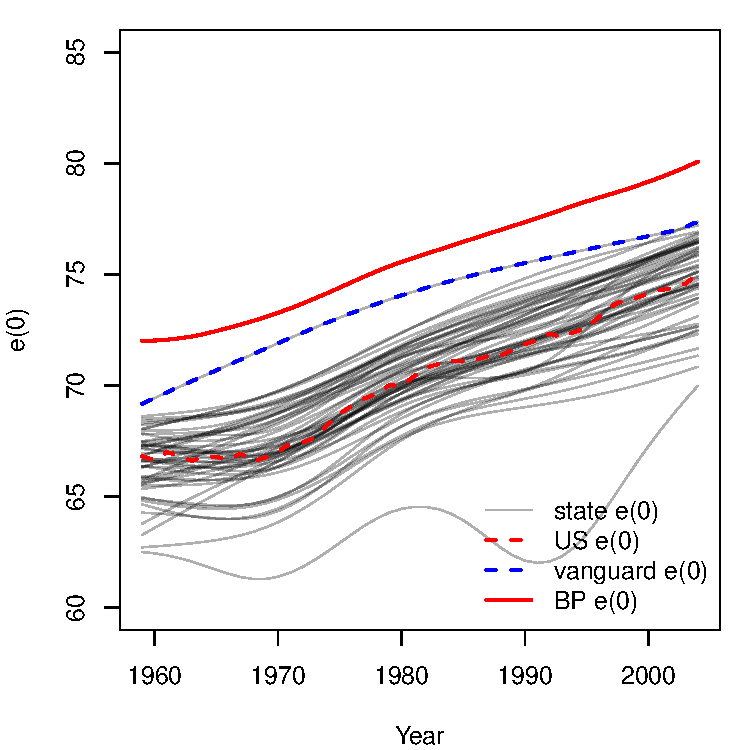
\includegraphics[scale=1.2]{Figures/e0trendsM.pdf}
    %\caption{Males (1959-2004\ldots)}
\end{figure} 
\end{frame}

\begin{frame}
\frametitle{Females (1959-2004, 12 causes)}
\begin{figure}[b]
    \centering
    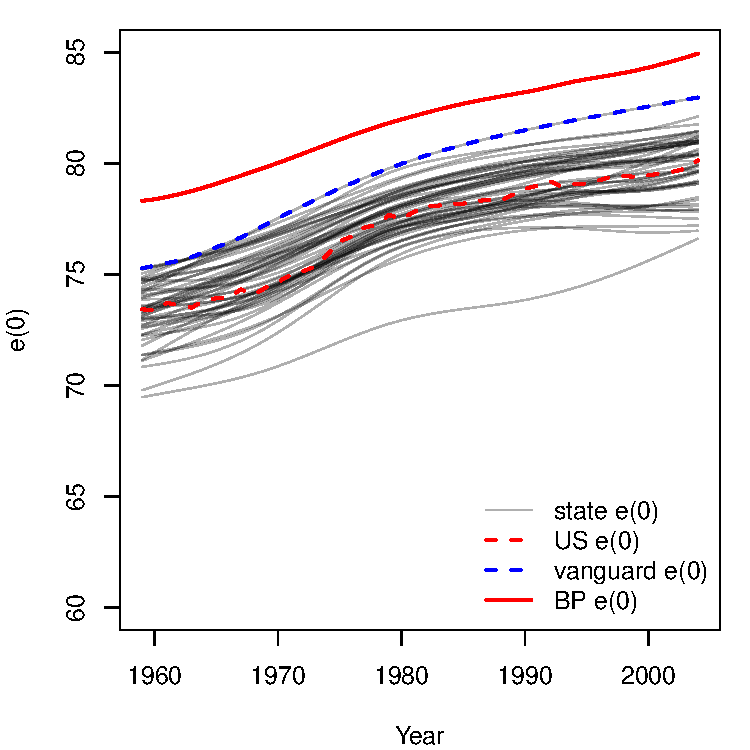
\includegraphics[scale=1.2]{Figures/e0trendsF.pdf}
    %\caption{Females (1959-2004\ldots)}
\end{figure} 
\end{frame}

\begin{frame}
\frametitle{Why do I care?}
\begin{block}{I: Regular}
Low mortality benchmark is the straightest line. It rose a steady 0.18/yr for
males, 0.15/yr for females. USA $e(0)$ runs 30 years behind.
\end{block}
\begin{block}{II: Lazy interpretation}
Achievable via pure diffusion
(technology, health care access, risk factors) and no other kind of progress.
\end{block}
\begin{block}{III: Endogenous reference}
Record life expectancy (Japan\ldots) is used as a sign of the future.
Low mortality benchmark is a reference closer to home, difussion easier to imagine.
\end{block}
\end{frame}

\begin{frame}
\frametitle{Why do I care?}
\begin{block}{IV: Endogenous reference}
Seriously, some projection proposals use Japan as a guide\ldots
\end{block}
\begin{figure}[b]
    \centering
    \includegraphics[scale=.8]{Figures/Pascariu.png}
    %\caption{Females (1959-2004\ldots)}
\end{figure} 
\end{frame}

\begin{frame}
\frametitle{Why do I care?}
\begin{block}{IV: Endogenous reference}
Seriously, some projection proposals use Japan as a guide\ldots
\end{block}
\begin{figure}[b]
    \centering
    \includegraphics[scale=.8]{Figures/Medford.png}
    %\caption{Females (1959-2004\ldots)}
\end{figure} 
\end{frame}

\begin{frame}
\frametitle{Digression}
\begin{quote}
A feature of counterfactuals is that they aren't true.
\end{quote}
\end{frame}


\begin{frame}
\frametitle{Digression}
\begin{quote}
Period $e(0)$ is a counterfactual too, ergo \textbf{fake}, but useful.\\
Is it so bad to do fake things with the components of $e(0)$?
\end{quote}
\end{frame}


\begin{frame}
\frametitle{Digression}
\begin{quote}
After all, it is the case that \\
``If a cohort of individuals were subjected to
the mortality rate schedule implied by the low-mortality benchmark (minimum
aggregation), then the average length of life would be LMB $e(0)$.''
\end{quote}
\end{frame}

\begin{frame}
\frametitle{So why not do cool stuff with LMB?}
State gap in $e(0)$ due to shortcomings in cardiovascular diseases
\begin{figure}[b]
    \centering
    \includegraphics[scale=1.2]{Figures/Cardio.pdf}
    %\caption{Females (1959-2004\ldots)}
\end{figure} 
\end{frame}

\begin{frame}
\frametitle{So why not do cool stuff with LMB?}
Or: potential increase in $e(0)$ given lowest \textit{presently
achievable} $\mu^{cardio}$.
 \begin{figure}[b]
    \centering
    \includegraphics[scale=1.2]{Figures/Cardio.pdf}
    %\caption{Females (1959-2004\ldots)}
\end{figure} 
\end{frame}

\begin{frame}
\frametitle{What's next?}
\begin{itemize}
\item Redo with 30 causes, through 2014. AP-smoothing of causes is tougher with
30 causes because there are many zero counts. Practical tips there would be
nice.
\item We're leaning towards an easy-to-chew public health article rather than a
demographic methods spin. The method can be sufficiently expressed in
one or two sentences, nothing fancy here.
\item If it were a methods paper, might make sense to compare with a lifetable
eliminated of causes \textit{amenable to treatment}.
\item Poster at PAA (P1-85, early morning Thursday\ldots)
\end{itemize}
\end{frame}
%\begin{frame}
%\begin{itemize}
%  \item\item<1-> Chrono variation = mortality morbidity tradeoff
%  \item\item<2-> Thano variation = win
 % \item\item<3-> miscategorizing thano variation leads in wrong direction
%  \item\item<4-> assumptions were strong here\ldots
%\end{itemize}
%\end{frame}
%%%%%%%%%%%%%%%%%%%%%%%%%%%%%%%%%%
%%	End of the document					%%
%%%%%%%%%%%%%%%%%%%%%%%%%%%%%%%%%%
\end{document}










